\chapter{Introduction to load balancing and RAID controllers}
\label{chap2:title}
\nomenclature{RAID}{Redundant Array of Independent Disks}
\nomenclature{ATA}{Serial ATA (AT Attachment)}
\nomenclature{IDE}{Integrated Drive Electronics}
\nomenclature{SAS}{Serial attached SCSI}
\nomenclature{SMART}{Self-Monitoring, Analysis and Reporting Technology}
\nomenclature{JBOD}{Just a Bunch of Disks}

In this chapter, we will focus on basic information for understanding the topic of the paper. We will discuss different types of load balancing systems and consider the things, which programmer should take into attention during implementation this kind of systems. This chapter also describes different types of RAID, which is very important topic, when we speak about the controllers. Finally, the last section tells about different write commands, which we use for the erasure of disks. This section gives the information about the structure of the commands and opens many command parameters in details. This chapter gives the basic knowledge for understanding the results of the thesis.

\newpage
\section{Load balancing}
In general, load balancing is the methodology that increases the speed by balancing the resources. This part of computer science is quite new, but the scientists started to focus on that almost 30 years ago \cite{stat_load_bal_1985}. The main idea is to do as much as possible with least amount of resources. Mostly it depends on the processes, which we can divide by threads and launch them parallel. Sometimes load balancing divides to the four types: static, dynamic, combined, and preemptive. In scientific articles, combined and preemptive load balancing systems are mentioned very rarely because of their specificity and usefulness only in some certain cases. That is why in this research we will consider two main different types: static and dynamic.
% combined? (http://masters.donntu.edu.ua/2011/fknt/baluta/library/article1.htm)
% preemptive? (http://dictionary.reference.com/browse/load+balancing)

Static load balancing system makes the analysis before the application starts to work. That is why the programmer should know some information for creating good load balancing system via static methods. Firstly, he should know the amount of distributed resources before starting the implementation of the program. Secondly, the programmer should divide the time in such a way that the duration of the tasks would be approximately the same. There are several methods to hand out the tasks such as Round Robin algorithm, Random algorithm, Recursive Bisection algorithm and some others \cite{oper_sys_conc}, \cite{perf_dlba}. Scientists frequently take the initial parameters from the previous launch results and genetic algorithms are used. We can take an example of load balancing system from image processing. Let consider 16$\times$16 segmented image and eight processors. With that image, each processor would work on four segments. The most important piece of all this division of work is that each processor determines this information and which segments it will work on.
\newpage
Dynamic load balancing systems have more possibilities than static systems because the balancing process can be done during the application running \cite{guide_dyn_bal}. This fact gives the advantage of resource movement from busy part to less busy. Thus, we will achieve that all parts of the application will be in average busy condition, which is the ideal solution. The disadvantage of this method is that the system should also collect the information about the status of application, which follows the increasing of the resources. The programmer should follow on three general criteria during implementation the dynamic load balancing system:
\begin{enumerate}%[topsep=0pt, itemsep=-0.5ex]
	\setlength{\itemsep}{-2mm}
%	\setlength{\topsep}{-10mm}
	\item Which process is busy or free 
	\item Priority of the task to be done 
	\item Length and/or duration of the task
\end{enumerate}
The program, which realizes the dynamic load balancing system, should check the loading of computation units, connection possibility, and frequency of sending commands. Dynamic load balancing technique has many methods, such as Bidding algorithm, Drafting algorithm \cite{draft_alg}, Recursive Coordinate Bisection (RCB) and some others. In this paper, we will call these methods as strategies, but it is also possible to find them in the literature as policies and logics.

\newpage
\section{RAID}
RAID - Redundant Array of Independent Disks - is a storage technology that combines multiple disk drive components into a logical unit. That means that this technology gives a possibility to keep the information in a specific way. RAID controllers are the devices, which realize this technology. In simple words, computer without a RAID controller can see physical disks as logical disks without any difference. However, the computer will see only the logical disks, if the RAID controller is connected. Logical disks are definitely different in comparison with physical disks. Nevertheless, logical disks can be equal to physical if RAID controller is set in special mode called JBOD (Just Bunch of Disks). RAID controller takes all issues about creation of these logical disks.

There are several types of RAID: RAID 0, RAID 1, RAID 5, RAID 6 and some others \cite{which_raid}. These types of RAID are basic types of RAID, thus there are many other types, which also combine them together. For example, RAID 10 is actually combining of RAID 0 and RAID 1. Each type or architecture provides a different balance between the key goals: reliability and availability, performance, and capacity. That means that every RAID keeps the information in a different way. 

One of the huge advantages of using RAID is that if one of the disks breaks down others can recover the information on that disk. Not all RAID architectures support this functionality, but most of them do. Some types of RAID provide fault tolerance of even two drive failures (RAID 6).

Let consider some types of RAID more detailed. RAID 1 called also as "mirroring" is one of the main fundamental types of RAID, which refers to maintaining duplicate sets of all data on separate disk drives. There must be two disks in the configuration and there is a cost disadvantage as the usable capacity is half the number of available disks. RAID 1 provides cost-effective, high fault tolerance for configurations with two disk drives. The prototype of RAID 1 is presented on the Figure \ref{fig:raid1}.
\begin{figure}[h!]
\begin{center}
  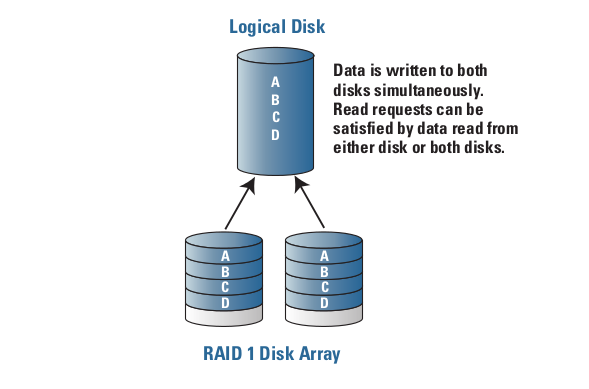
\includegraphics[width=0.95\textwidth]{raid1}
\end{center}
  \caption{Prototype of RAID 1}
  \label{fig:raid1}
\end{figure}

Another type RAID 5, which is presented on the Figure \ref{fig:raid5}, uses data striping in a technique designed to provide fault-tolerant data storage, but doesn't require duplication of data like RAID 1 \cite{raid_overview}. Data is striped across all of the drives in the array, but for each stripe through the array (one stripe unit from each disk), one stripe unit is reserved to hold parity data calculated from the other stripe units in the same stripe. Read performance is therefore very good, but there is a penalty for writes, since the parity data has to be recalculated and written along with the new data. RAID 5 requires a minimum of three disks and a maximum of 16 disks. RAID 5 usable capacity is between 67\% - 97\% depending on the number of data drives in the RAID set.
\begin{figure}[h]
\begin{center}
  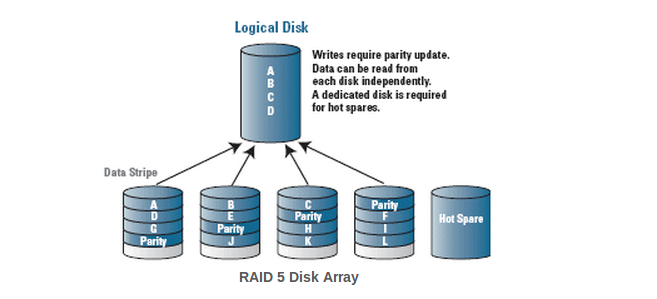
\includegraphics[width=0.95\textwidth]{raid5}
\end{center}
  \caption{Prototype of RAID 5}
  \label{fig:raid5}
\end{figure}
Moreover, nowadays there are RAID controllers, which already have load balancing system inside and the user can set the mode, which is more comfortable in the some situations. This system takes care only about logical disks, but we need to communicate only with physical disks. That is why we need to have our own load balancing system, which will help us to distribute the resources before the commands come to the controller. Because in our case the commands should be sent straight to the disks, load balancing system from the controller does not help at all. Moreover, during communication directly with the disks, we do not need to remember if there is any RAID or not, because the commands are sent through the controller without any changes.  

The Figure \ref{fig:3ware_RAID} presents one of the SATA RAID controllers. 
\begin{figure}[h]
\begin{center}
  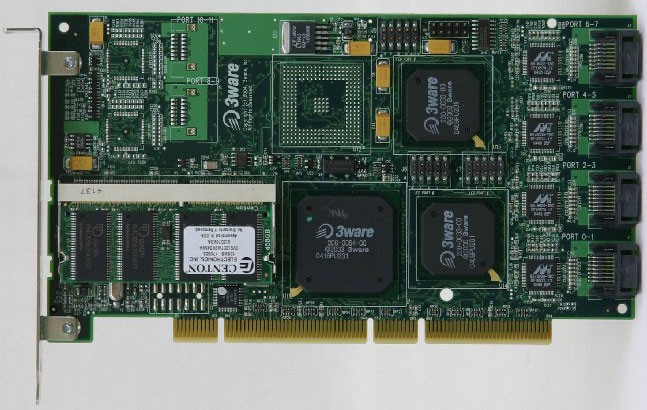
\includegraphics[width=0.95\textwidth]{3ware_RAID}
\end{center}
  \caption{3ware SATA RAID controller 9500S-8}
  \label{fig:3ware_RAID}
\end{figure}
From the name of the device, it is clear that this controller can be connected to 8 SATA disks. It supports following types of RAID: 0, 1, 5, 10, 50 and JBOD (Just a Bunch of Disks).

\newpage
\section{SCSI RAID controllers}
SCSI - Small Computer System Interface - is a set of standards for physically connecting and transferring data between computers and peripheral devices \cite{book_of_scsi}. The SCSI standards define commands, protocols, and electrical and optical interfaces. There are also other interfaces such as SATA (Serial ATA (AT Attachment)), IDE (Integrated Drive Electronics), SAS (Serial attached SCSI). In general, we divide the interfaces to two categories: ATA and SCSI. In the following content, it means the according protocol. IDE and SATA interfaces relate to ATA and SAS belongs to SCSI. Several types of disks are presented on the Figure \ref{fig:disks}. In this paper, the topic mostly is about SCSI interface, but sometimes we compare it with ATA. If we compare SAS and SCSI, we consider them as similar interfaces. However, SAS is a new version of SCSI and it gives a single channel for each disk. SCSI has only one channel for all disks.
\begin{figure}[h]
  \advance\leftskip-0.1\textwidth
  \subfloat[SCSI disk]{
    \label{fig:scsi}
    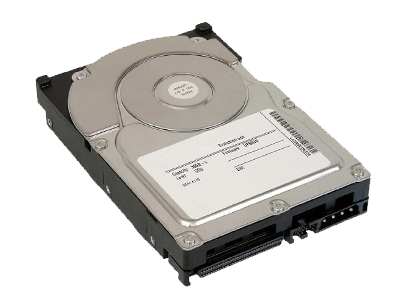
\includegraphics[width=0.6\textwidth]{scsi}
  }
  \subfloat[SATA and IDE disks]{
    \label{fig:sata_ide_disks}
    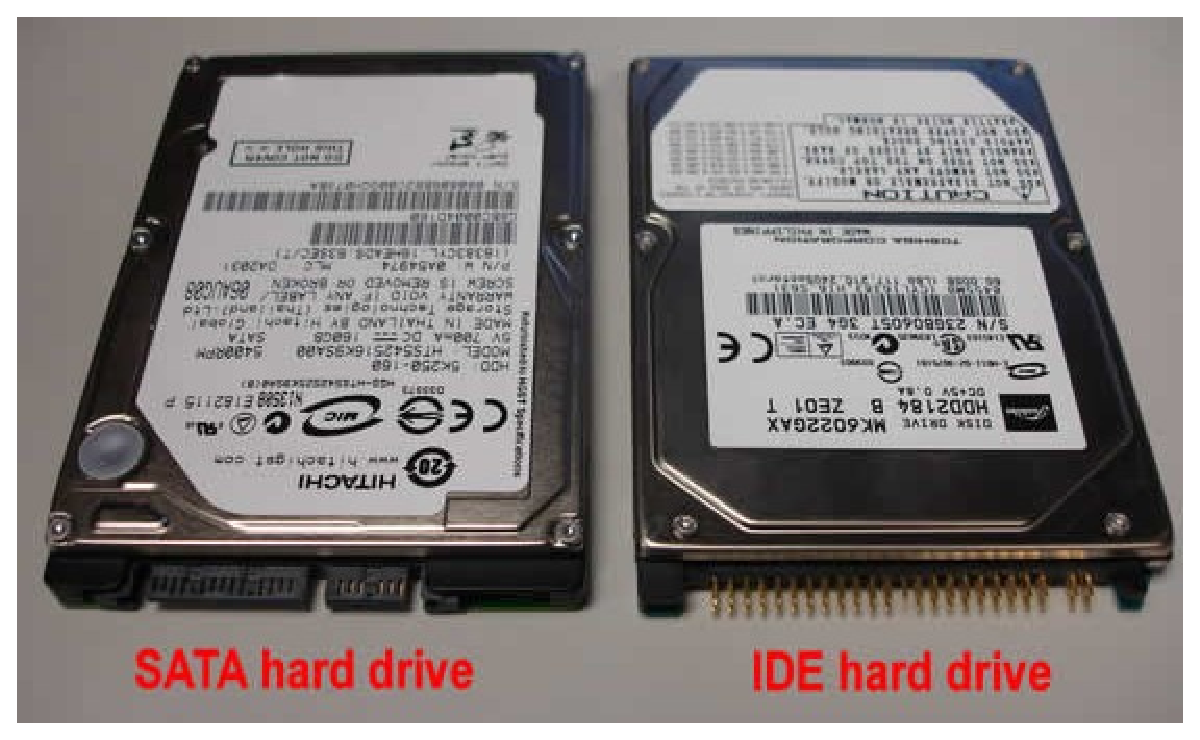
\includegraphics[width=0.6\textwidth]{sata_ide_disks}
  }
  \caption{Three different types of disks}
  \label{fig:disks}
\end{figure}

\section{SCSI WRITE and WRITE SAME commands}
\label{subsec:write_comm}
This research is made for the Blancco Oy Ltd, which produce the erasure software. The main part of the erasure is performed by SCSI WRITE and WRITE SAME commands \cite{scsi3_bc}. In general, all commands belongs to three groups: Non-Data commands, Data-In and Data-Out. For the last two groups it means that the programmer should send the command including the buffer. Data-Out means that the data is sent to the disk. For the Data-In group it is in opposite way and data comes from the disk. The example of Data-In command is any SCSI READ command. Write commands belongs to the Data-Out group because these commands must have Data-Out buffer, containing the data, which we write to the disk. Nowadays, for SCSI there are 4 different versions of write command and 3 for the write same command.  

Lets consider SCSI WRITE commands first. Mostly the commands are different because of the length. Each command has not only operation code, which is the main criteria for the command, but also some other variables such as Logical Block Address (LBA), transfer length, control and some others. These variables do not include Data-Out buffer and the Figure \ref{fig:write_10} shows the example how the commands are defined in specification \cite{scsi3_bc}.
\begin{figure}[h]
\begin{center}
  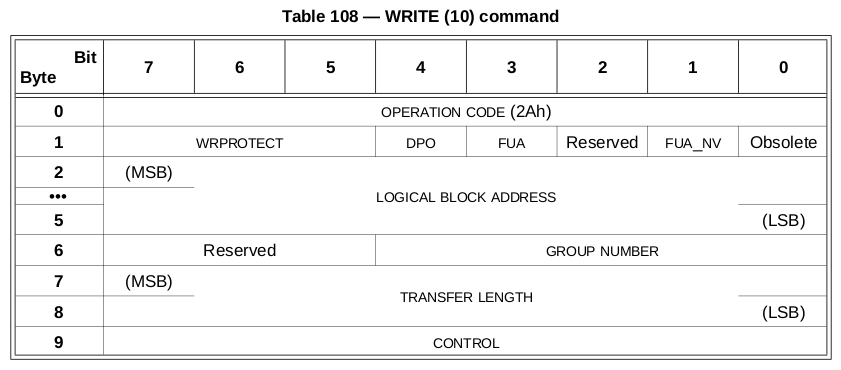
\includegraphics[width=0.95\textwidth]{write_10}
\end{center}
  \caption{Definition of WRITE 10 command}
  \label{fig:write_10}
\end{figure}

The following commands exist for writing the data to the disk:
\begin{itemize}%[topsep=0pt, itemsep=-0.5ex]
	\setlength{\itemsep}{-2mm}
%	\setlength{\topsep}{-10mm}
	\item WRITE (10)
	\item WRITE (12)
	\item WRITE (16)
	\item WRITE (32)
\end{itemize}
The numbers in brackets shows the length of the command in bytes. It is obvious that the WRITE (10) command is the base for others. It seems that by now the best choice is WRITE (16) because in \cite{scsi3_bc} there are some notes, that <<Migration from the WRITE (10) command to the WRITE (16) command is recommended for all implementations>>. WRITE (32) should be used only in some special cases \cite{scsi3_bc}. In this research, we will focus only on WRITE 10 command, because after some test, it started to be understandable, that bus plays an important role in this model, and there is no reason to send more data.

SCSI WRITE SAME commands have the same purposes as SCSI write commands. The difference and biggest advantage is that SCSI WRITE SAME command can be sent once and the Data-Out buffer can be written to the disk several times. That gives faster speed because the bus is not busy any more - only one command was sending, but the buffer is still writing. 

There are three different types of write same commands, as we mentioned before:
\begin{itemize}
	\setlength{\itemsep}{-2mm}
	\item WRITE SAME(10)
	\item WRITE SAME(16)
	\item WRITE SAME(32)
\end{itemize}
The number in brackets also shows the length of the command in bytes. Number of logical blocks is one of the most important variables in these commands because we write this number of blocks to the disk with the same buffer. It is obvious that if the length of the SCSI WRITE SAME command is quite big, we can write to the disks much more number of blocks. We will consider only WRITE SAME 10 command, because the results after few tests showed that there is no reason to send bigger buffer, because the disk could not work faster. ATA specification has the similar command, but it should be send differently and the device should support SMART (Self-Monitoring, Analysis and Reporting Technology) \cite{ata_spec}. It is a monitoring system for computer hard disk drives to detect and report on various indicators of reliability.

